%% Direttive TeXworks:
% !TeX root = ../../maltoni_niccolo_tesi.tex
% !TEX encoding = UTF-8 Unicode
% !TEX program = arara
% !TEX TS-program = arara
% !TeX spellcheck = it-IT

\chapter{Background}\label{ch:background}
    \section{Alchemist}\label{sec:alchemist}
        Alchemist\footnote{\url{http://alchemistsimulator.github.io}}~\cite{alchemist2013} è un meta-simulatore estendibile completamente \engEmph{open-source} che esegue su \engEmph{Java~Virtual~Machine} (JVM), nato all'interno dell'Università di Bologna e distribuito su licenza GNU GPLv3+ con \engEmph{linking exception};
        il codice è reperibile su GitHub\footnote{\url{https://github.com/AlchemistSimulator/Alchemist}}, dove chiunque fosse interessato può collaborare sviluppando nuove estensioni, migliorando funzionalità esistenti e risolvendo possibili bug.

        \subsection{Introduzione ad Alchemist}\label{subsec:introAlchemist}
            In generale, una \emph{simulazione}~\cite{des3} è una riproduzione del modo di operare di un sistema o un processo del mondo reale nel tempo.
            L'imitazione del processo del mondo reale è detta \emph{modello};
            esso risulta essere una riproduzione più o meno semplificata del mondo reale, che viene aggiornata ad ogni passo di esecuzione della simulazione.

            Alchemist rientra nell'archetipo dei simulatori ad eventi discreti (DES)~\cite{des, des2}:
            gli eventi sono strettamente ordinati e vengono eseguiti uno alla volta, determinando il passare del tempo.
            L'idea dietro al progetto è quello di riuscire ad avere un framework di simulazione il più possibile generico, in grado di simulare sistemi di tipologia e complessità diverse, mantenendo le prestazioni dei simulatori non generici (come ad esempio quelli impiegati in ambito chimico~\cite{gillespie1976}).

            Per perseguire questo obiettivo, la progettazione dell'algoritmo è partita dallo studio del lavoro di Gillespie del 1977~\cite{gillespie1977} e di altri scienziati nell'ambito della simulazione chimica.
            Nonostante siano presenti algoritmi in grado di eseguire un numero di reazioni addirittura in tempo costante, la scelta dell'algoritmo è infine ricaduta su una versione migliorata dell'algoritmo SSA di Gillespie, il Next Reaction Method~\cite{nextReactionMethod} di Gibson e Bruck:
            ad ogni passo di simulazione, esso è in grado di selezionare la reazione successiva in tempo costante e richiede un tempo logaritmico per aggiornare le strutture dati interne al termine dell'esecuzione dell'evento.

        \subsection{Astrazioni e modello di Alchemist}\label{subsec:modello}
            Il modello di astrazione di Alchemist è ispirato dal lavoro della comunità scientifica nell'ambito dei simulatori a scopo di ricerca chimica e ne riprende dunque la nomenclatura.
            Le entità (visibili in \Cref{fig:model}) su cui lavora sono le seguenti:

            \begin{description}
                \item[Molecola]\label{itm:mol}
                    Una \emph{Molecola} rappresenta il nome dato ad un particolare dato all'interno di un \emph{Nodo}, del quale ne astrae parte dello stato.

                    Un parallelismo con la programmazione imperativa vedrebbe la \emph{Molecola} come un'astrazione del nome di una variabile.

                \item[Concentrazione]\label{itm:conc}
                    La \emph{Concentrazione} di una \emph{Molecola} è il valore associato alla proprietà rappresentata dalla \emph{Molecola}.

                    Mantenendo il parallelismo con la programmazione imperativa, la \emph{Concentrazione} rappresenterebbe il valore della variabile.

                \item[Nodo]\label{itm:node}
                    Il \emph{Nodo} è un contenitore di \emph{Molecole} e \emph{Reazioni} che risiede all'interno di un \emph{Ambiente} e che astrae una singola entità.

                \item[Ambiente]\label{itm:env}
                    L'\emph{Ambiente} è l'astrazione che rappresenta lo spazio nella simulazione ed è l'entità che contiene i \emph{Nodi}.

                    Esso è in grado di fornire informazioni in merito alla posizione dei \emph{Nodi} nello spazio, alla distanza tra loro e al loro vicinato;
                    opzionalmente, l'\emph{Ambiente} può offrire il supporto allo spostamento dei \emph{Nodi}.

                \item[Regola di collegamento]\label{itm:linkr}
                    La \emph{Regola di collegamento} è una funzione dello stato corrente dell'\emph{Ambiente} che associa ad ogni \emph{Nodo} un \emph{Vicinato}.

                \item[Vicinato]\label{itm:neigh}
                    Un \emph{Vicinato} è un'entità costituita da un \emph{Nodo} detto ``centro'' e da un insieme di altri \emph{Nodi} (i ``vicini'').

                    L'astrazione dovrebbe avere un'accezione il più possibile generale e flessibile, in modo da poter modellare qualsiasi tipo di legame di vicinato, non solo spaziale.

                    \begin{figure}[htbp]
                        \centering
                        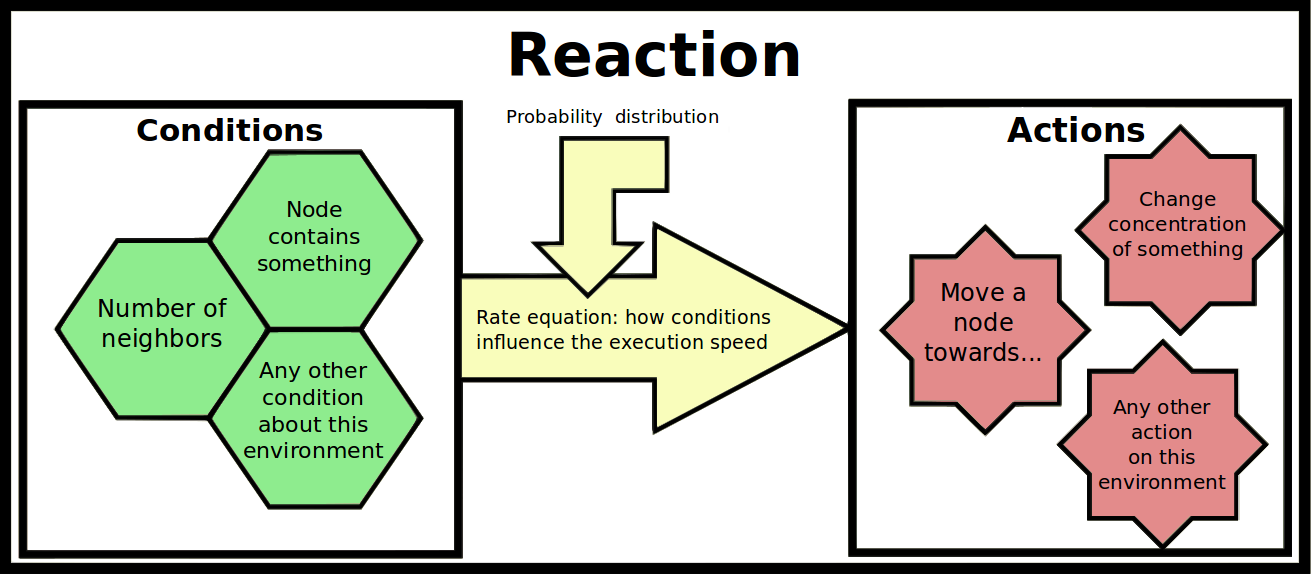
\includegraphics[scale=.35]{fig/alchemist_reaction}
                        \caption{%
                            La figura, rivisitata da quella disponibile sul sito ufficiale, offre una rappresentazione grafica della \emph{Reazione}.
                        }
                        \label{fig:react}
                    \end{figure}

                \item[Reazione]\label{itm:react}
                    Il concetto di \emph{Reazione} è da considerarsi molto più elaborato di quello utilizzato in chimica:
                    in questo caso, si può considerare come un insieme di \emph{Condizioni} sullo stato del sistema, che qualora dovessero risultare vere innescherebbero l'esecuzione di un insieme di \emph{Azioni}.

                    Una \emph{Reazione} (di cui è si ha una rappresentazione grafica in \Cref{fig:react}) è dunque un qualsiasi evento che può cambiare lo stato dell'\emph{Ambiente} e si compone di un insieme di \emph{Condizioni}, una o più \emph{Azioni} e una distribuzione temporale.

                    La frequenza di accadimento può dipendere da:
                    \begin{itemize}
                        \item[--] Un tasso statico;
                        \item[--] Il valore di ciascuna \emph{Condizione};
                        \item[--] Una equazione che combina il tasso statico e il valore delle \emph{Condizioni}, restituendo un ``tasso istantaneo'';
                        \item[--] Una distribuzione temporale.
                    \end{itemize}

                    Ogni \emph{Nodo} è costituito da un insieme (anche vuoto) di \emph{Reazioni}.

                \item[Condizione]\label{itm:cond}
                    Una \emph{Condizione} è una funzione che associa un valore numerico e un valore booleano allo stato corrente di un \emph{Ambiente}.

                \item[Azione]\label{itm:act}
                    Un'\emph{Azione} è una procedura che provoca una modifica allo stato dell'\emph{Ambiente}.

            \end{description}

            \begin{figure}[htbp]
                \centering
                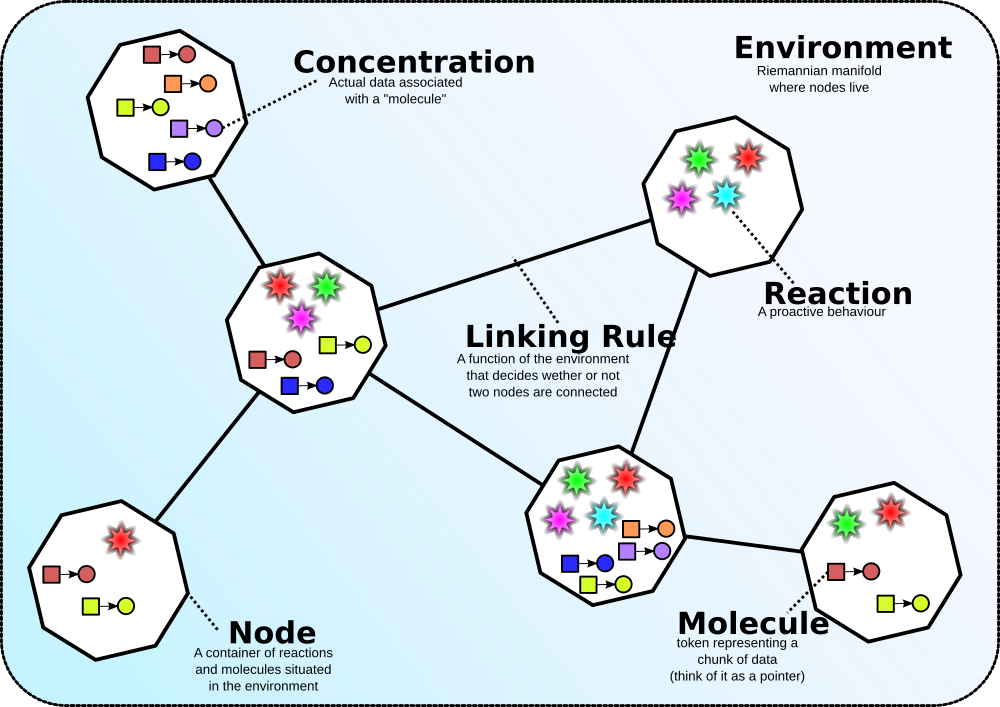
\includegraphics[scale=.4]{fig/alchemist_model}
                \caption{%
                    La figura, presa dal sito ufficiale, offre una rappresentazione grafica delle diverse entità.
                    All'interno di un ambiente, che modella il sistema, si trovano i nodi connessi tra loro attraverso dei collegamenti;
                    ogni nodo è composto da reazioni e molecole, ognuna delle quali ha associata una concentrazione.
                }
                \label{fig:model}
            \end{figure}

        \subsection{Interfaccia utente classica}\label{subsec:prevGui}
            L'architettura di Alchemist è progettata con paradigma \engEmph{Model-View-Controller}~\cite{mvc} (MVC), di conseguenza la suddivisione tra componente grafica (\engEmph{View}) e il blocco ``logico'' composto da \engEmph{Model} e \engEmph{Controller} è netta.
            Questa distinzione è evidente anche per quanto riguarda l'utilizzo pratico del software:
            una simulazione su Alchemist può venire lanciata da terminale, senza che alcuna interfaccia grafica sia necessaria per tutta la durata del periodo di esecuzione, oppure essere inizializzata, lanciata e controllata in tempo reale dalla sua interfaccia grafica.

            Per lo scopo di questa tesi, tratteremo esclusivamente della GUI.

            \subsubsection{Esperienza utente}\label{subsubsec:prevUx}
                Un'interfaccia grafica (detta anche GUI, \engEmph{graphical user interface}~\cite{gui}) è l'insieme dei componenti grafici con i quali l'utente può interagire per impartire comandi ad un programma del computer, che si contrappone ad un altro metodo di interazione, l'interfaccia a riga di comando (o CLI, \engEmph{Command Line Interface}).

                L'interfaccia grafica è stata ideata negli anni `80 a partire da un'esigenza di maggiore usabilità rispetto dalla riga di comando, derivante soprattutto dall'affermarsi degli studi di usabilità~\cite{norman1988} e di ergonomia cognitiva~\cite{cognitiveErgonomics} di quel periodo.

                Più ampio e moderno è invece il concetto di esperienza utente~\cite{ux} (spesso abbreviata in UX, \engEmph{User eXperience}):
                l'ISO 9241-210~\cite{iso9241} la definisce come ``le percezioni e le reazioni di un utente che derivano dall'uso o dall'aspettativa d'uso di un prodotto, sistema o servizio''.
                Di fatto, essa descrive la reazione dell'utente di fronte all'interazione con il programma o lo strumento in base a tre dimensioni:
                \begin{itemize}
                    \item[--] \emph{Dimensione pragmatica}:
                        funzionalità e usabilità del sistema;
                    \item[--] \emph{Dimensione estetica/edonistica}:
                        piacevolezza estetica, emotiva e ludica del sistema;
                    \item[--] \emph{Dimensione simbolica}:
                        attributi sociali, forza del brand, identificazione.
                \end{itemize}
                L'usabilità, invece, fa riferimento unicamente ai soli aspetti pragmatici (la capacità di svolgere un compito con efficienza ed efficacia).

                L'interfaccia utente classica di Alchemist è caratterizzata da un'usabilità appena sufficiente, funzionale alle necessità di un utilizzatore esperto, ma non adeguata a fornire un'esperienza completa e \engEmph{user-friendly} ad un utente ``standard''.

                Grazie a contributi recenti~\cite{casadio}, la GUI ha subito un parziale rinnovamento, limitato alla parte di ambiente integrato che accoglie l'utilizzatore che stia lanciando il simulatore senza una simulazione specificata;
                questa parte non è oggetto del lavoro illustrato in questa tesi.
                Al contrario, è interessante analizzare lo stato dell'interfaccia relativa all'ambiente di esecuzione della simulazione.

                La criticità principale, che va a minare non solo il livello di esperienza utente, ma anche il concetto di usabilità  ``classico'', è evidente nella non intuitività dei controlli:
                come è possibile vedere in \Cref{fig:oldMain}, non sono presenti bottoni di interazione per, ad esempio, avviare o fermare la simulazione o per cambiare la modalità di interazione con la zona in cui viene rappresentato l'ambiente;
                questo perché molte possibilità di controllo sono limitate a scorciatoie da tastiera non modificabili e non descritte altrove se non nella documentazione.

                \begin{figure}[htbp]
                    \centering
                    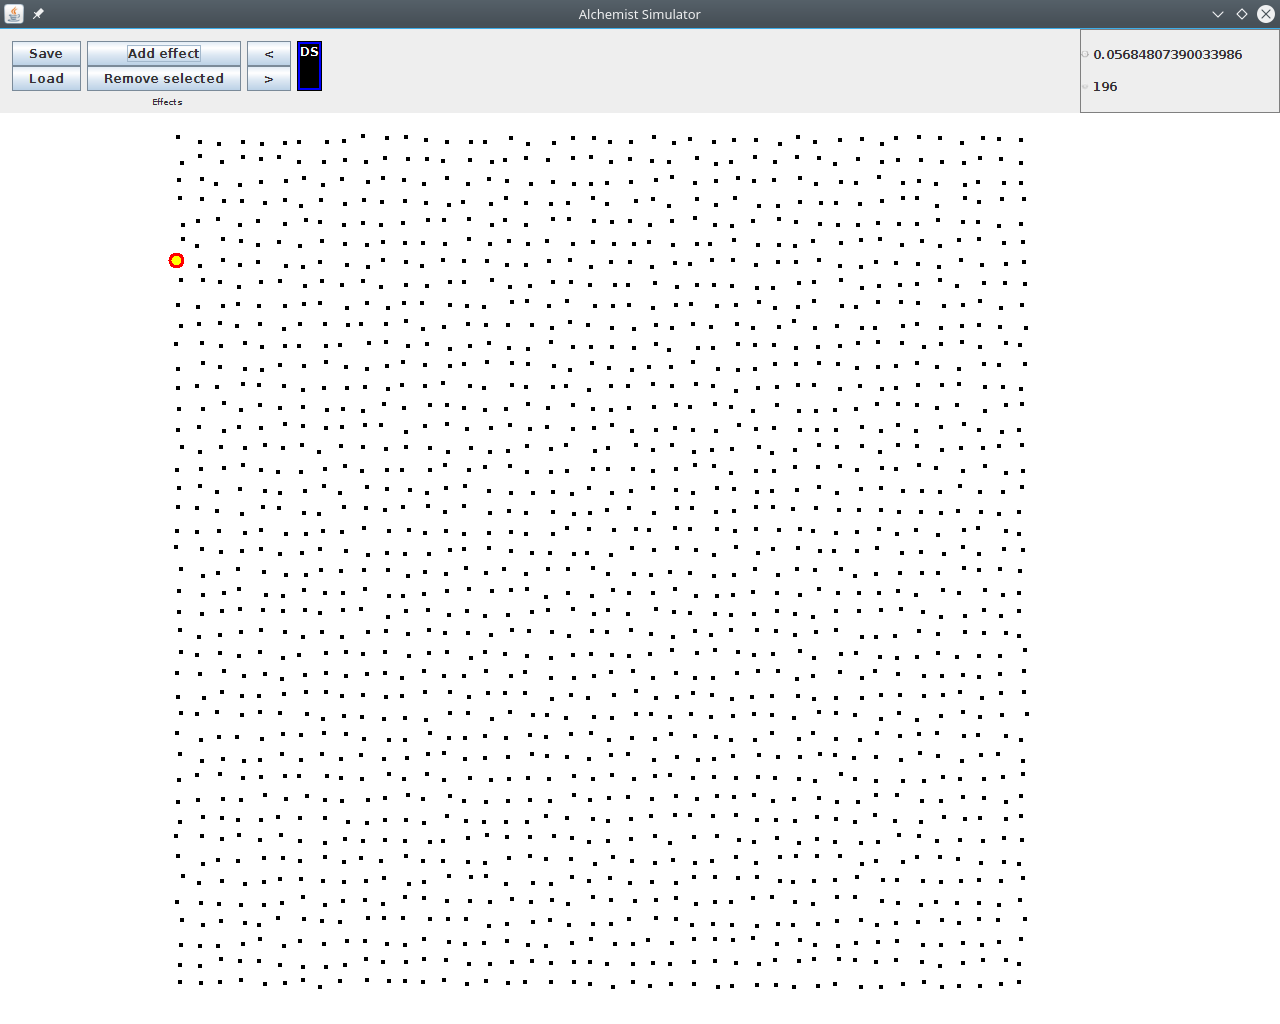
\includegraphics[scale=.35]{old/window_started}
                    \caption{Vista principale di una simulazione con l'interfaccia classica}
                    \label{fig:oldMain}
                \end{figure}

                Un'ultima criticità che esula dal contesto pratico, ma che rientra appieno nel contesto estetico importante per una buona UX è, appunto l'aspetto grafico:
                l'intera interfaccia di simulazione è implementata sfruttando le impostazioni di base del framework Swing, senza alcun tipo di personalizzazione al \engEmph{look'n'feel} che potesse identificare uno stile originale di Alchemist, né che lo allineasse alle direttive di un design grafico ben definito (come il Material Design\footnote{\url{https://material.io}} di Google o Modern UI e Fluent Design System\footnote{\url{https://fluent.microsoft.com}} di Microsoft), né che si adattasse al \engEmph{look'n'feel} standard del sistema operativo.

            \subsubsection{Swing}\label{subsubsec:swing}
                Come detto, Alchemist utilizza Swing come strumento per implementare l'interfaccia grafica.
                Java Swing è un framework per lo sviluppo di GUI in Java, parte delle \engEmph{Java Foundation Classes} (JFC) insieme ad AWT (\engEmph{Abstract Window Toolkit}) e \emph{Java 2D}.

                Come è possibile vedere in \Cref{fig:awt}, la libreria sfrutta i componenti forniti da AWT, mettendone a disposizione di nuovi in grado di risolvere diverse debolezze del precedente standard grafico per il linguaggio di Oracle:

                \begin{figure}[htbp]
                    \centering
                    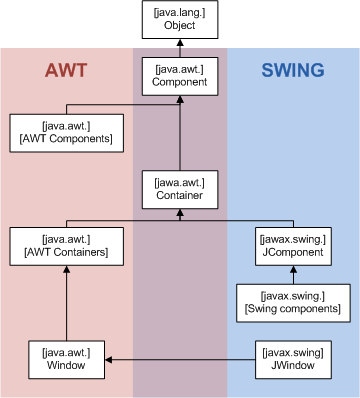
\includegraphics[scale=.45]{fig/awt_swing}
                    \caption{Struttura delle classi di Swing e AWT}
                    \label{fig:awt}
                \end{figure}

                \begin{itemize}
                    \item[--]
                        Swing è molto più facilmente estendibile e rende possibile un controllo della presentazione grafica dei componenti (il \engEmph{look'n'feel}) trasparente, non necessitando più di classi specifiche per ogni aspetto grafico.
                    \item[--]
                        I componenti forniti da Swing permettono inoltre di realizzare un'interfaccia più leggera di quella di AWT:
                        essa sfrutta infatti le API fornite da Java 2D, anziché chiamare il \engEmph{toolkit} di interfacce native del sistema operativo;
                        nel contempo, appoggiandosi al container di AWT, sfrutta l'accesso al framework di gestione delle GUI fornito dall'OS, traducendo gli eventi specifici dell'OS in eventi Java disaccoppiati dalla piattaforma su cui gira la JVM, semplificando la gestione da parte dello sviluppatore.
                    \item[--]
                        Swing rende più semplice appoggiarsi al pattern MVC per implementare software con GUI, separando le classi di modello da quelle grafiche e di controllo.
                \end{itemize}

            \subsubsection{Gli effetti}\label{subsubsec:effect}
                Una parte consistente della visualizzazione di una simulazione di Alchemist, nell'interfaccia classica come in quella attuale, è costituita dagli effetti.

                Concettualmente, in Alchemist un \emph{effetto} è una rappresentazione grafica di ``qualcosa'' nell'ambiente;
                costituisce di fatto una modalità semplificata per l'utente di cogliere quanto accade nella simulazione.

                L'effetto classico si presenta  come una funzione dal nodo all'interfaccia grafica:
                esso è in grado di rappresentare qualsiasi proprietà di un nodo dato, ma non può riferirsi se non marginalmente alle altre entità dell'ambiente.

    \section{JavaFX}\label{sec:jfx}
        Nel mese di maggio del 2007 alla conferenza annuale JavaOne, Sun Microsystems annunciò JavaFX Script (chiamato anche F3, \engEmph{Form~Follows~Function}), un DSL (\engEmph{Domain~Specific~Language}, linguaggio di dominio specifico) pensato per lo sviluppo di interfacce grafiche di Rich Internet Applications~\cite{moritz2008rich}, e JavaFX Mobile, un sistema software per dispositivi mobili basato su Java e ispirato all'allora neonato iPhone, che avrebbe avuto come cavallo di battaglia la possibilità di sviluppare app mobile in grado di condividere codice e asset grafici con le controparti desktop e web, semplificando lo sviluppo di ecosistemi strutturati.

        Incluso nella versione 1.0 del pacchetto JavaFX rilasciato nel dicembre del 2008, JavaFX Script venne però abbandonato da Oracle (che nel frattempo aveva acquisito Sun Microsystems) meno di 2 anni dopo, in contemporanea con l'ampliamento della disponibilità delle JavaFX API agli altri linguaggi disponibili per JVM;
        anche JavaFX Mobile, con l'avvento di OS mobili moderni come Android e iOS, è considerato deprecato.

        JavaFX continua invece lo sviluppo come framework per la gestione di interfacce grafiche per Java ed altri linguaggi JVM-compatibili, andando di fatto a sostituire Swing e AWT.

        In questo capitolo si intende analizzare il framework e le sue funzionalità fino alla versione utilizzata nella stesura del codice, nonché l'ultima versione stabile all'atto di inizio del lavoro illustrato in questa tesi:
        JavaFX 8.

        \subsection{Introduzione al framework JavaFX}\label{subsec:jfxIntro}
            La prima versione di JavaFX ad abbandonare JavaFX Script e JavaFX Mobile, con i quali il framework era nato, per andare ad affiancarsi a Swing è la versione 2.0, distribuita parzialmente su licenza \engEmph{open-source} verso la fine del 2011.
            Essa introduceva un nuovo linguaggio XML dichiarativo, l'FXML, in grado di fornire una struttura grafica all'applicazione coinvolgendo minimamente il codice Java, oltre a migliorare il supporto \engEmph{multi-thread}.
            Con le successive versioni 2.1 e 2.2, rilasciate nell'arco del 2012, fu esteso il supporto a MacOS e Linux.

            La prima versione ad essere parte del JRE/JDK è JavaFX 8, rilasciata il 18 marzo 2014 insieme a Java 8;
            essa diventa di fatto la nuova libreria di riferimento per lo sviluppo di applicazioni grafiche per ambiente JVM.

            Essa si presenta come fortemente orientata verso i pattern di progettazione \engEmph{Model-View-Controller} e \engEmph{Model-View-Presenter};
            la suddivisione infatti è netta:
            \begin{itemize}
                \item[--]
                    La \emph{componente visiva} è definita su file di markup FXML, logicamente separati da qualsiasi componente Java che non siano le loro classi \engEmph{Controller};
                    anche la \emph{presentazione}, definibile attraverso fogli di stile CSS, è indipendente dalle altre componenti Java e XML e può essere anche sostituita a tempo di esecuzione senza difficoltà;
                \item[--]
                    Il \emph{controllo} dell'applicazione è circoscritto a classi Java specifiche, che vengono associate al caricamento del documento di markup corrispondente;
                    per design sono facilmente sostituibili da differenti implementazioni progettate per interagire con gli oggetti che il parser di JavaFX riconosce nel file FXML;
                \item[--]
                    In una implementazione che sfrutti appieno gli strumenti messi a disposizione del framework, per design il \emph{modello} non viene coinvolto dalle suddette componenti e resta dunque distaccato dalle suddette componenti.
            \end{itemize}

            Oltre al già citato miglioramento per quanto riguarda il \engEmph{look'n'feel} (che ora può vantare la semplificazione data dai fogli di stile CSS), un ulteriore flessibilità grafica è il supporto Hi-DPI, che permette alle GUI di adattarsi a schermi ad elevata densità di pixel.

        \subsection{Architettura del framework JavaFX}\label{subsec:jfxFramework}
            Come è possibile osservare in \Cref{fig:jfxArch}, l'architettura interna di JavaFX è costituita da diversi livelli, ciascuno dei quali sfrutta le funzionalità messe a disposizione dai livelli inferiori per offrire nuove API ai livelli superiori e allo sviluppatore finale.

            Il livello più elevato per la costruzione di una applicazione JavaFX è il grafo delle scene (\engEmph{Scene Graph}):
            esso ospita un albero gerarchico di nodi, ciascuno dei quali rappresentante un elemento visivo dell'interfaccia utente.
            Questo livello si occupa anche di intercettare gli input e di mettere a disposizione le JavaFX API pubbliche.

            Un singolo elemento del grafo delle scene è chiamato \emph{nodo}.
            Ogni nodo possiede un ID, una classe di stile e un volume delimitato;
            fatta eccezione per il nodo radice, ogni nodo possiede un solo nodo genitore e può essere a sua volta genitore di uno o più altri nodi.
            Su ogni nodo possono essere definiti effetti grafici (come blur e ombre) e livello di opacità, nonché stati specifici per l'applicazione e comportamenti in caso di eventi specifici.

            Il livello subito inferiore allo \engEmph{Scene Graph} è costituito dal \engEmph{JavaFX Graphics System} (in \Cref{fig:jfxArch} è rappresentato dagli elementi in azzurro), che attraverso il \engEmph{Quantum Toolkit} e \engEmph{Prism} mette a disposizione funzionalità più a basso livello per rappresentazioni 2D e 3D.

            I processi di \engEmph{Prism} si occupano del rendering;
            possono eseguire sia con accelerazione hardware che senza e sono in grado di realizzare sia rendering 2D che 3D.
            Attraverso questi processi vengono eseguite le rasterizzazioni e i rendering di tutti i grafi delle scene.

            Il \engEmph{Quantum Toolkit} collega invece \engEmph{Prism} al \engEmph{Glass Windowing Toolkit} e gestisce le regole di threading per rendering e gestione degli eventi.

            \begin{figure}[htbp]
                \centering
                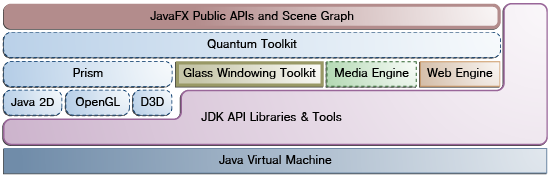
\includegraphics[scale=0.75]{fig/jfx_arch}
                \caption[La figura, presa dalla documentazione ufficiale di Oracle, rappresenta i diversi livelli che caratterizzano il framework JavaFX]{La figura, presa dalla documentazione ufficiale di Oracle\protect\footnotemark, rappresenta i diversi livelli che caratterizzano il framework JavaFX}
                \label{fig:jfxArch}
            \end{figure}
            \footnotetext{\url{https://docs.oracle.com/javase/8/javase-clienttechnologies.htm}}

            Il terzo livello è costituito dal sopra citato \engEmph{Glass Windowing Toolkit}, che rappresenta il livello più basso del \engEmph{JavaFX Graphics Stack}.
            Esso si occupa di gestire i servizi nativi forniti dai sistemi operativi per la gestione delle finestre e delle code degli eventi;
            costituisce la parte \engEmph{platform-dependent} di JavaFX.

            \engEmph{Media Engine} e \engEmph{Web Engine} si occupano del supporto per i file multimediali audiovisivi e per i linguaggi web.

        \subsection{Struttura di una Applicazione JavaFX}\label{subsec:jfxStruttura}

            JavaFX fornisce le classi di base per strutturare una applicazione completa, delimitando linee guida ben specifiche nella suddivisione della struttura.

            \begin{figure}[htbp]
                \centering
                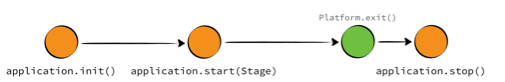
\includegraphics[scale=1]{fig/jfx_lifecycle}
                \caption{La figura rappresenta il ciclo di vita di una applicazione JavaFX}
                \label{fig:jfxLife}
            \end{figure}

            La classe principale per una applicazione JavaFX deve estendere da \texttt{javafx\dothyp application\dothyp Application}.
            Il metodo \texttt{start()} è il punto di ingresso principale:
            lanciando una JavaFX Application attraverso il metodo \texttt{launch()} della classe di supporto \texttt{javafx\dothyp application\dothyp Platform}, verrà inizializzato il framework e poi verranno chiamati in ordine i metodi \texttt{init()} e \texttt{start(javafx\dothyp stage\dothyp Stage)}, che rappresentano di fatto il ciclo di inizializzazione ideale dell'applicazione.
            Il metodo \texttt{main()} non deve essere necessariamente implementato perché l'applicazione possa essere avviata:
            esso viene infatti creato dal \engEmph{JavaFX Packager Tool} durante l'inserimento del \engEmph{JavaFX Launcher} nel file JAR.

            Il layout con cui un'applicazione JavaFX è costituita a livello grafico si struttura gerarchicamente su tre sezioni principali, visibili in \Cref{fig:jfxStage}:

            \begin{description}
                \item[\texttt{Stage}]\label{itm:stg}
                    In JavaFX, una finestra è astratta tramite la classe \texttt{javafx\dothyp stage\dothyp Stage}:
                    letteralmente ``\emph{palcoscenico}'',  è il contenitore di livello più elevato e funge da ``guscio esterno'' per ogni altro componente grafico e pannello.

                    Lo \texttt{Stage} primario viene costruito dalla piattaforma all'atto di avvio, ma ulteriori \texttt{Stage} possono venire costruiti durante l'esecuzione, purché attraverso il \engEmph{JavaFX Application Thread}.

                    \begin{figure}[htbp]
                        \centering
                        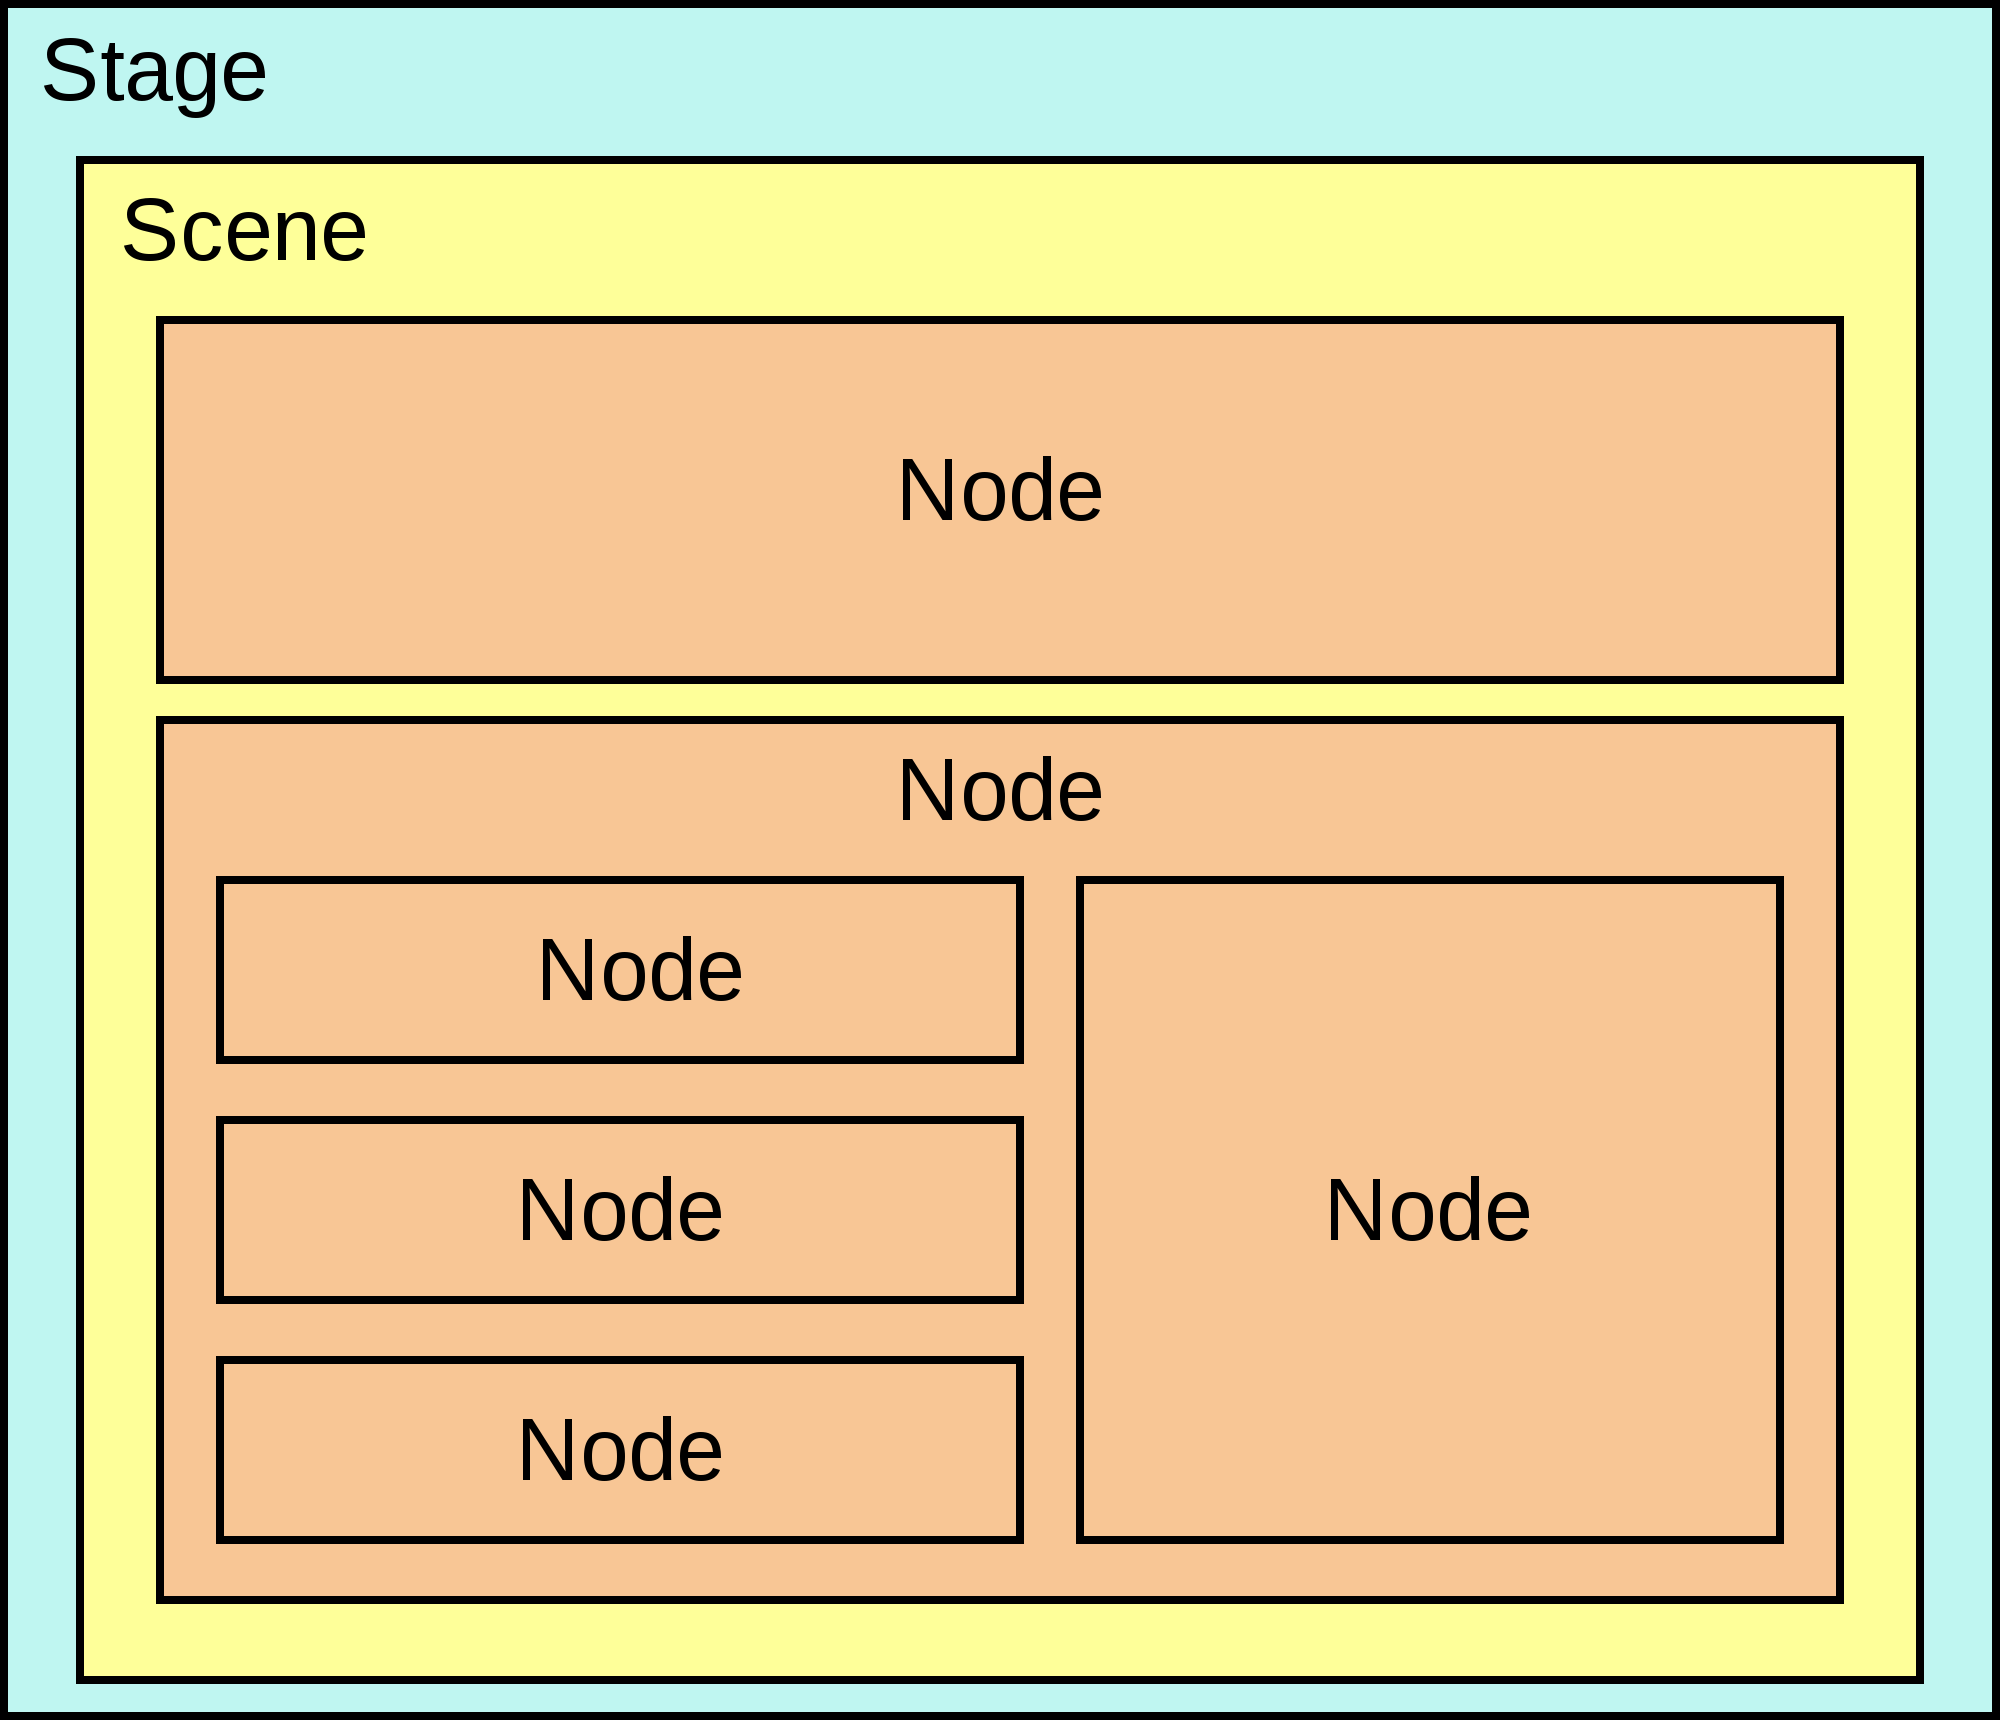
\includegraphics[scale=0.12]{fig/jfx_stage_scene_node}
                        \caption{Struttura del layout di una applicazione JavaFX}
                        \label{fig:jfxStage}
                    \end{figure}

                \item[\texttt{Scene}]\label{itm:scn}
                    Il contenuto dello \texttt{Stage} è rappresentato dalla classe \texttt{javafx\dothyp scene\dothyp Scene}, che è a sua volta contenitore di ogni nodo appartenente a quello specifico \engEmph{Scene Graph}.

                \item[\texttt{Pane}]\label{itm:pane}
                    Come già affermato nella \Cref{subsec:jfxIntro}, ogni elemento appartenente ad una \emph{scena} è detto \emph{nodo}.
                    Il terzo livello è costituito da un particolare tipo di nodo, detto \emph{pannello} (modellato dalla classe \texttt{javafx\dothyp scene\dothyp layout\dothyp Pane}), che costituisce il contenuto di una scena e gestisce la disposizione dei nodi al suo interno sullo schermo;
                    è possibile costruire una struttura gerarchica inserendo all'interno di un pannello radice altri pannelli.

                \item[\texttt{Node}]\label{itm:nod}
                    La classe \texttt{javafx\dothyp scene\dothyp Node} modella ogni singolo componente dello \engEmph{Scene Graph}, dai già citati pannelli ai bottoni, canvas, campi di testo e così via.

                    In \Cref{fig:jfxNode} è possibile vedere una rappresentazione gerarchica delle diverse tipologie di \emph{nodo}.
            \end{description}

            \begin{figure}[htbp]
                \centering
                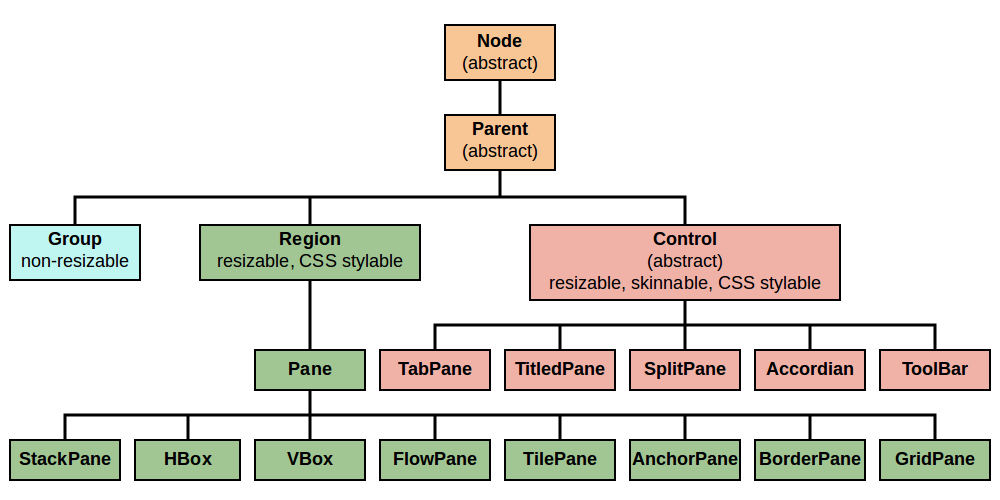
\includegraphics[scale=0.4]{fig/jfx_layout_classes}
                \caption{Struttura dei nodi di JavaFX}
                \label{fig:jfxNode}
            \end{figure}

        \subsection{JavaFX e Swing a confronto}\label{subsec:jfxVantaggi}

            \begin{figure}[hbpt]
                \centering
                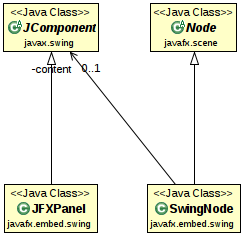
\includegraphics[scale=0.8]{uml/jfxSwingAdapt}
                \caption{Diagramma delle classi \engEmph{adapter} per \emph{nodi JavaFX} e \emph{componenti Swing}}
                \label{fig:jfxSwingAdapt}
            \end{figure}

            Nonostante sia presente un livello di interoperabilità fornito dalle classi \engEmph{adapter} \texttt{JFXPanel} e \texttt{SwingNode} del package \texttt{javafx\dothyp embed\dothyp swing} (\Cref{fig:jfxSwingAdapt}), come già sostenuto nella \Cref{subsec:jfxIntro} lo sviluppo del framework JavaFX è orientato prima ad affiancare poi a sostituire Swing e le \engEmph{Java Foundation Classes} come ambiente grafico per applicazioni su \engEmph{Java Virtual Machine}.

            Escludendo il fatto di essere la libreria grafica non di terze parti più moderna per Java e il cosiddetto ``\engEmph{eye candy factor}'', JavaFX può vantare diversi vantaggi su Swing:

            \begin{description}
                \item [FXML]\label{itm:fxml}
                    L'utilizzo di un linguaggio di markup basato su XML per la definizione della componente di UI offre un approccio dichiarativo nel processo di costruzione che Swing non poteva offrire;
                    inoltre, questo porta ad un incapsulamento della componente \engEmph{View} dei pattern di progettazione MV* sostanzialmente ``automatico''.

                    Da non sottovalutare è anche la presenza di un software ufficiale per il design dell'interfaccia in FXML:
                    \engEmph{Scene Builder}.
                    Esso offre un'interfaccia \engEmph{drag'n'drop} per l'aggiunta dei componenti grafici ed è integrato in tutti gli ambienti di sviluppo più utilizzati (Eclipse, Intellij IDEA, Netbeans).
                    La versione più recente del software creato da Oracle è distribuito da Gluon\footnote{\url{http://gluonhq.com/products/scene-builder}}.

                \item[Skin e CSS]\label{itm:css}
                    Altro miglioramento in merito alla flessibilità riguarda il supporto ai fogli di stile CSS (\engEmph{Cascading Style Sheet}):
                    ampiamente utilizzati nello sviluppo web, essi permettono di sviluppare temi per una applicazione JavaFX senza coinvolgere il codice Java, a differenza dei \engEmph{look'n'feel} di Swing, né i file FXML, incapsulando completamente la componente di presentazione.

                \item[Supporto multimediale]\label{itm:media}
                    Grazie a JavaFX Media, la piattaforma supporta nativamente i più comuni formati audio (MP3, AIFF, WAV, AAC) e video (FLV con compressione VP6, MP4 con compressione H.264/AVC) senza richiedere l'utilizzo di librerie esterne.
                    Il supporto è incluso anche nella \engEmph{Webview}.

                \item[Animazione]\label{itm:anim}
                    Rispetto a Swing, il supporto alle animazioni (sia per quanto riguarda il movimento di componenti grafiche che gli effetti di transizione) è stato notevolmente alleggerito;
                    è stato inoltre introdotto il supporto alle alterazioni regolate dal tempo, precedentemente molto complesse da implementare a causa del paradigma di rappresentazione tramite doppio buffer di default.

                \item[Supporto HTML]\label{itm:html}
                    Completamente assente in Swing era la possibilità di rendering di contenuti HTML;
                    con JavaFX è stato inserito il supporto completo a Javascript, HTML5 e CSS tramite motore di rendering WebKit (utilizzato da browser come Safari, Google Chrome e Opera) e nodi \texttt{Webview} dedicati.

                \item[Scaling e Hi-DPI]\label{itm:hidpi}
                    Recentemente si sta verificando un progressivo innalzarsi delle densità degli schermi:
                    sono sempre più comuni display 4K UltraHD anche di piccole dimensioni, che possono causare problemi di visualizzazione ad applicazioni con interfacce non progettate per una grande varianza di risoluzioni e densità di pixel.
                    Infatti, l'utilizzo di valori assoluti per quanto riguarda la dimensione dei componenti grafici rende la GUI molto piccola e soprattutto quasi totalmente inutilizzabile dall'utente, a causa dell'elevato rapporto di pixel per unità di dimensione.

                    JavaFX 8 introduce il supporto a Hi-DPI, assente in Swing.
            \end{description}

    \section{Interfaccia JavaFX per Alchemist: motivazioni}\label{sec:motivi}
        Come spiegato nella \Cref{subsubsec:prevUx}, l'esperienza utente dell'interfaccia utente classica di Alchemist è estremamente limitata.
        Miglioramenti recenti~\cite{casadio} sono stati apportati a parte dell'interfaccia, impiegando la libreria JavaFX per implementare un'esperienza d'uso più intuitivo, simile all'utilizzo di un IDE.
        Evidente era dunque la necessità di una nuova interfaccia grafica per l'ambiente di simulazione, che potesse avvicinare utilizzatori meno esperti in ambito informatico all'utilizzo dei Alchemist per impieghi scientifici nei loro campi di competenza.

        Si è scelto dunque di effettuare la reimplementazione in JavaFX anche per questa parte per diversi motivi:

        \begin{itemize}
            \item[--]
                Poiché l'alternativa valutabile era Swing, la prima motivazione è composta da tutte le nuove funzionalità elencate nella \Cref{subsec:jfxVantaggi};
                in particolare, era importante il supporto ad uno scaling corretto dell'interfaccia su tutti gli schermi e una gestione delle animazioni più leggera che potesse impattare in modo inferiore le risorse della macchina e lasciare maggiore potenza computazionale al motore di simulazione.

                Inoltre, è stato considerato interessante l'orientamento ``intrinseco'' che l'utilizzo di file FXML ha verso il pattern MVC, già utilizzato in Alchemist per il design della struttura dei moduli.

            \item[--]
                Una seconda motivazione riguarda il supporto futuro:
                come illustrato precedentemente, JavaFX si presenta come il nuovo punto di riferimento per quanto riguarda l'implementazione di GUI per applicazioni JVM, dunque è stato considerato più conveniente abbandonare la soluzione \engEmph{legacy} Swing per la più nuova alternativa.

            \item[--]
                In ultimo, vi è una motivazione prettamente estetica:
                la maggiore flessibilità a livello di personalizzazione grafica che JavaFX è in grado di offrire ha permesso di adottare le direttive grafiche di design molto apprezzati come, in questo caso, il Material Design definito da Google.
        \end{itemize}
